\documentclass{article}
\usepackage[utf8]{inputenc}
\usepackage{graphicx}
\usepackage[a4paper, total={6in, 9in}]{geometry}
\usepackage{amsmath}
\usepackage{mathtools}
\usepackage{steinmetz}
\usepackage{float}
\DeclarePairedDelimiter\evaluat{.}{\rvert}
\reDeclarePairedDelimiterInnerWrapper\evaluat{nostar}{\mathopen{}#2\mathclose{#3}}
\DeclarePairedDelimiter\abs{\lvert}{\rvert}%
\DeclarePairedDelimiter\norm{\lVert}{\rVert}%
\usepackage{pgfplots}
\usepackage{pst-plot}

 
\title{ELEC344 Assignment 2}
\author{Name: Brendan Lai, Student Number: 19241173}
\date{Due: March 28, 2021}
  
\begin{document}
  
\maketitle
  
\tableofcontents

\section{Question 1}
Using the buck converter provided and the following conditions solve each part:
\begin{center}
\begin{tabular}{ c   c }
    $V_{in} = 48V$ & $C = 400 \mu F$\\ 
    $V_{out} = 12V$ &  $R = 10 \Omega$\\  
    $L = 10 mH$ & $f_{sw} = 10kHz$    
\end{tabular}
\end{center}

\section*{Part a:}
Based on the desired input-output voltage ratio, calculate the duty cycle $D$.\\
\\
Analyze the ratio between the desired output voltage and the input voltage. Further we know that $V_{out} = D *V$ so we can therefore derive that:\\
\begin{align*}
    D = \frac{V_{out}}{V_{in}} = \frac{12}{48} \xrightarrow[]{} D = 0.25. \\
\end{align*}

\section*{Part b:}
Calculate the average, maximum and minimum values of the wave forms.
\begin{center}
\begin{tabular}{ c   c }
    Inductor voltage & Capacitor current\\ 
    Inductor current &  Output Voltage\\  
    Input Current\\    
\end{tabular}
\end{center}
\\ To calculate these values we must make a few assumptions:
\begin{center}
    \begin{tabular}{c   c}
    efficiency = 100\% & $V_{in} \geq V_{out}$ \\
    Ripple voltage $<<$ average output voltage & We're analyzing steady state \\
    \end{tabular}
\end{center}
Considering state 1 (S1 closed, S2 open) calculate the voltage across the inductor for "T-on". At state 2 (S2 open, S1 closed) we get "T-off" \\
\\ Firstly, state 1:
\begin{align*}
    V_L(t) &= L \frac{di_L}{dt} = V_{on} - \Bar{V_0} \\
    i_L(t) &= C \frac{dV_0}{dt} = i_L - i_0,\mbox{ where $i_0 = \frac{\Bar{V_0}}{R} = \Bar{Z_0}$}
\end{align*}
\\ Similarly, in state 2:
\begin{align*}
        V_L(t) &= L \frac{di_L}{dt} = 0 - \Bar{V_0} \\
    i_L(t) &= C \frac{dV_0}{dt} = i_L - \Bar{Z_0}
\end{align*}
\\First looking at calculating the inductor voltage we know that the maximum is in state 1 while the minimum is at state 2: 
\begin{align*}
    V_{L,max} &= V_i - V_0 = 48 - 12 = 36V \\
    V_{L,min} &= 0 - 12 = -12V \\
    V_{L,avg} &= \frac{48-12}{2} = 12V
\end{align*}
\\ Next looking at the Inductor current we use state two to find the change in current (V source disconnected). Thus we see:
\begin{align*}
    \Delta i_L = -\frac{V_0 (1-D)}{L*f_{sw}} = 12 * \frac{1-0.25}{(10*10^{-3})(10*10^3)} = 0.09A
\end{align*}
\\Also, average inductor current is described by: $I_L = \frac{V_0}{R} = \frac{12}{10} = 1.2A$
\\Thus, we can calculate the minimum and maximum of the values at steady state:
\begin{align*}
    I_{L,max,min} &= I_L \pm \Delta i_L / 2 \\
    I_{L,max,min} &= 1.2 \pm \frac{0.09}{2} = 1.245A, 1.155 A
\end{align*}
\\To calculate the output voltage we use $\Delta Q = C*\DeltaV$ and know that the capacitor voltage will be a triangular waveform. Therefore we get that:
\begin{align*}
    \Delta Q = \frac{1}{2}*\frac{T}{2}*\frac{\Delta i_L}{2}\\
    \rightarrow \Delta V_0 &= \frac{\Delta I_L}{8*C*f_{sw}} = \frac{0.09}{8*400*10^{-6}*10*10^3} = 0.00281V
\end{align*}
\\Average output voltage is 12V as given from the question therefore $V_{0,max,min} = V_0 \pm \Delta V_0$
\begin{align*}
    V_{0,min} &= V_0 - \frac{\Delta V_0}{2} = 12 - \frac{0.00281}{2} = 11.999V\\
    V_{0,max} &= V_0 + \frac{\Delta V_0}{2} = 12 - \frac{0.00281}{2} = 12.001V
\end{align*}
\\ To find the capacitor current, we know that at steady state the current is zero. Therefore $i_{C,avg} =0$. The input current can be found using KCL and we know that the maximum and minimum capacitor currents can be found at state 1 and 2 respectively.
\begin{align*}
    i_{C,max} &= i_L - i_0 = i_L - \frac{V_{0,avg}}{R} = 1.245 - \frac{12}{10} = 0.045A \\
    i_{C,min} &= i_L - i_0 = i_L - \frac{V_{0,avg}}{R} = 1.155 - \frac{12}{10} = -0.045A 
\end{align*}
\\Finally, calculating the input current we know it is the same as the inductor current at state 1 and zero at state 2 as the source is disconnected.
\begin{align*}
    i_{in,max} &= 1.245A \\
    i_{in,min} &= 1.245A \\
    i_{in,avg} &= i_{in,max} * D = 1.245*0.25 = 0.311A
\end{align*}
\\Moreover, the following table describes the full results and it can be found in the following section where it can be compared to the simulated results:

\section*{Part c:}
Simulate the buck converter shown in Figure 1 in PSIM. Plot the following wave forms. Compare the average maximum and minimum values of the waveforms obtained from your calculations and simulation results. Make relevant comments on the results.
\begin{figure}[H]
    \centering
    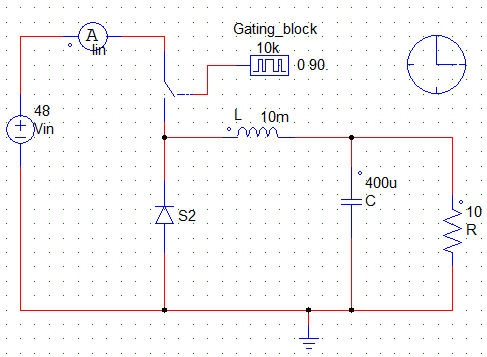
\includegraphics[width=0.75\textwidth]{q1c-ciricuit.png}
    \caption{q.1c circuit}
\end{figure}
\\The figures for the following circuit can all be found on "here" page:
\begin{figure}[H]
    \centering
    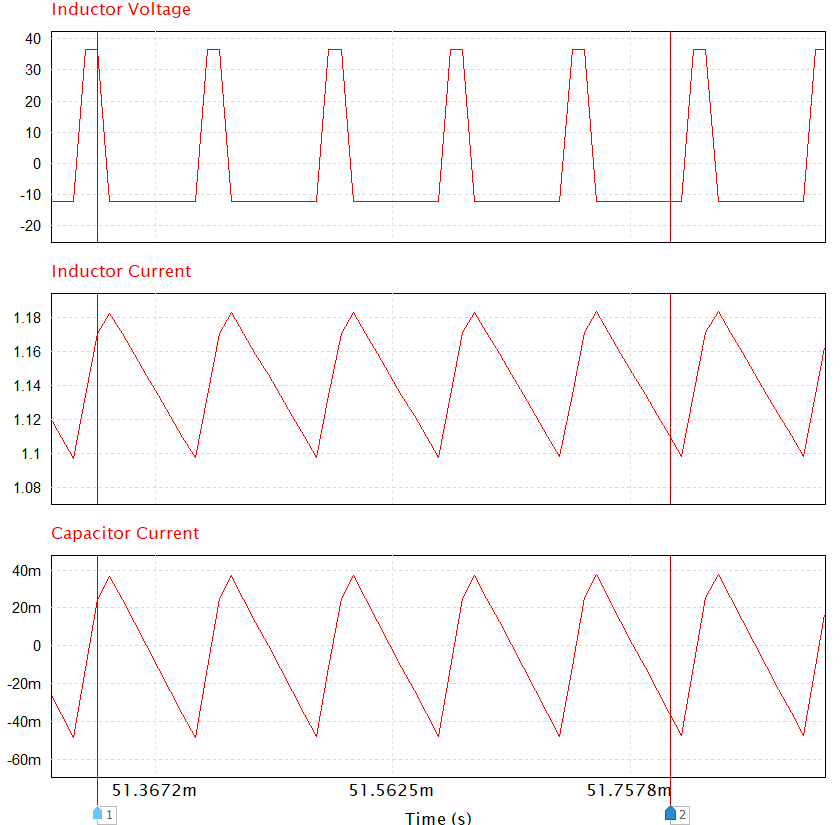
\includegraphics[width=0.65\textwidth]{q1c-f1.png}
    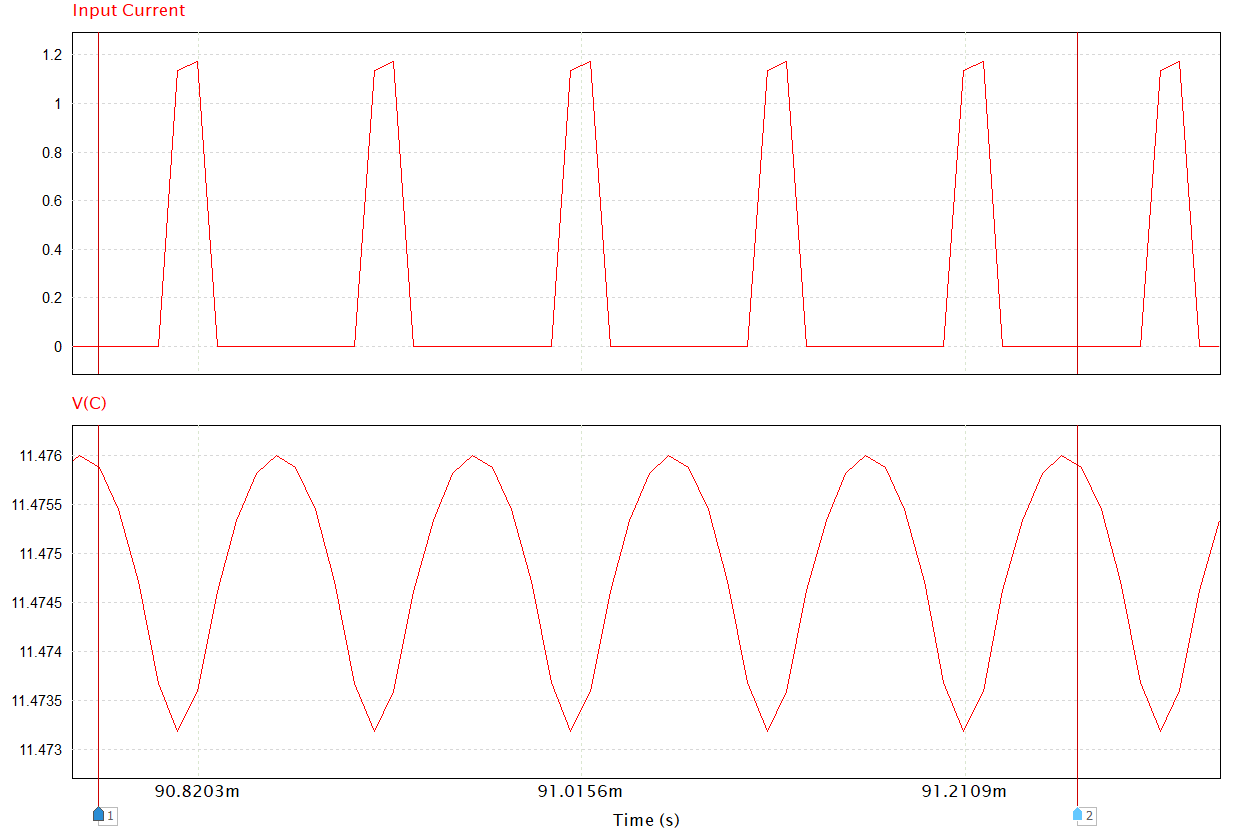
\includegraphics[width=0.65\textwidth]{q1c-f2.png}\\
    \caption{Waveforms for Q1c}
\end{figure}

\\The results from the measured simulations and the theoretical calculations were as follows:

\begin{center}
 \begin{tabular}{|c |c c c c c||} 
 \hline
  Theoretical & $V_L$[V]& $i_L$ [A] & $i_C$ [A] & $V_0$ [V] & $i_{in}$ [A] \\ [0.5ex] 
 \hline\hline
 min & -12 & 1.155 & -0.045 & 11.999 & 0 \\ 
 \hline
 max & 36 & 1.245 & 0.045 & 12.001 & 1.245\\
 \hline
 average & 12 & 1.2 & 0 & 12 & 0.311 \\
 [1ex] 
 \hline
\end{tabular}
\end{center}

\begin{center}
 \begin{tabular}{|c |c c c c c||} 
 \hline
  Simulated & $V_L$[V]& $i_L$ [A] & $i_C$ [A] & $V_0$ [V] & $i_{in}$ [A] \\ [0.5ex] 
 \hline\hline
 min & -12.01 & 1.13 & -0.0478 & 11.998 & 0 \\
 \hline
 max & 36.13 & 1.25 & 0.0446 & 12.001 & 1.253\\
 \hline
 average & 12.14 & 1.19 & 0 & 12 & 0.626 \\
 [1ex] 
 \hline
\end{tabular}
\end{center}

\section*{Part d:}
While the circuit is running, the load resistance changes to $R = 5 \Omega$. Plot ht waveforms of the transient in PSIM and explain qualitatively why the capacitor voltages shows a dip right after the load transient.
\begin{figure}[H]
    \centering
    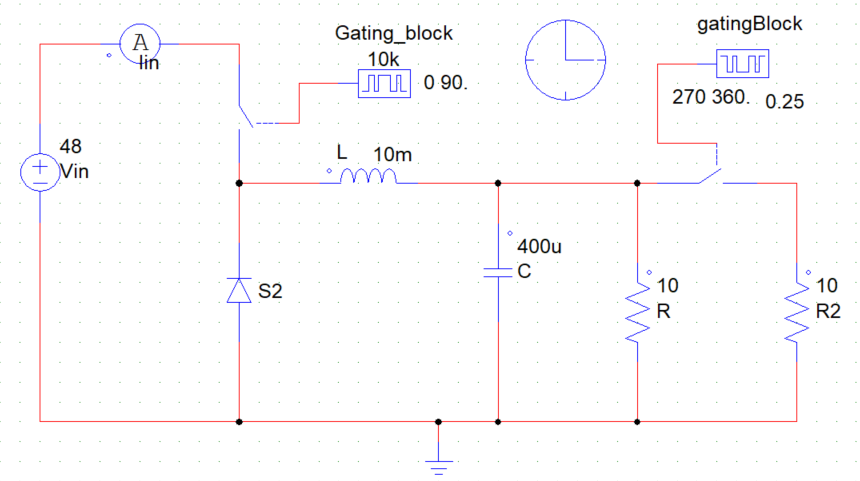
\includegraphics[width=0.65\textwidth]{q1d.png}\\
    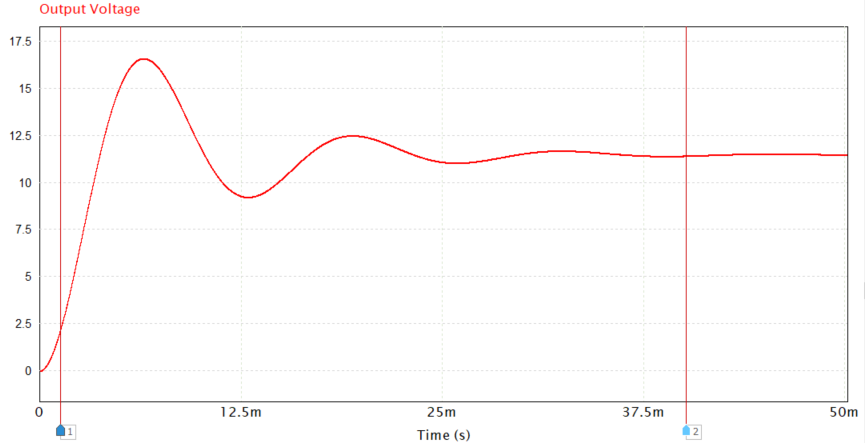
\includegraphics[width=0.65\textwidth]{q1d-f.png}
    \label{Figures for Q1c}
\end{figure}
\\Here we see that after applying the load that output voltage drops because the added load limits the amount of current that can flow. An analogy to this would be if you think about when you're drinking bubble tea (if you ever do). When drinking bubble tea if there is a pearl (boba) coming up the straw less liquid is coming through since the boba acts as a block. Further when you're not drinking any of the pearls you get more liquid to drink. Moreover, in our case when there is no boba more liquid can pass and similarly at a lower resistance more current flows. Ultimately, the decrease in charge on the capacitor reduce the voltage, which leads to the dip as they are directly proportional.

\section*{Part e:}
The engineer wants to change the switching frequency to $f_{sw} = 100Hz$. Would you recommend proceeding with this change? Why?\\
\\A higher switch frequency yields a smoother DC output. By decreasing the switching frequency to 100Hz from 10kHz the ripple in the output voltage would significantly increase which we would prefer not to happen. As a result, by changing the switching frequency we would increase the ripple by several magnitudes which is undesirable. 

\section{Question 2}
The magnetic circuit shown is formed by two TDK E 25/13/7 cores made of N87 material with g=0.55 mm (total air-gap 1mm). The core and magnetic material data sheets can be found in the assignment sheet.\\
\begin{figure}[H]
    \centering
    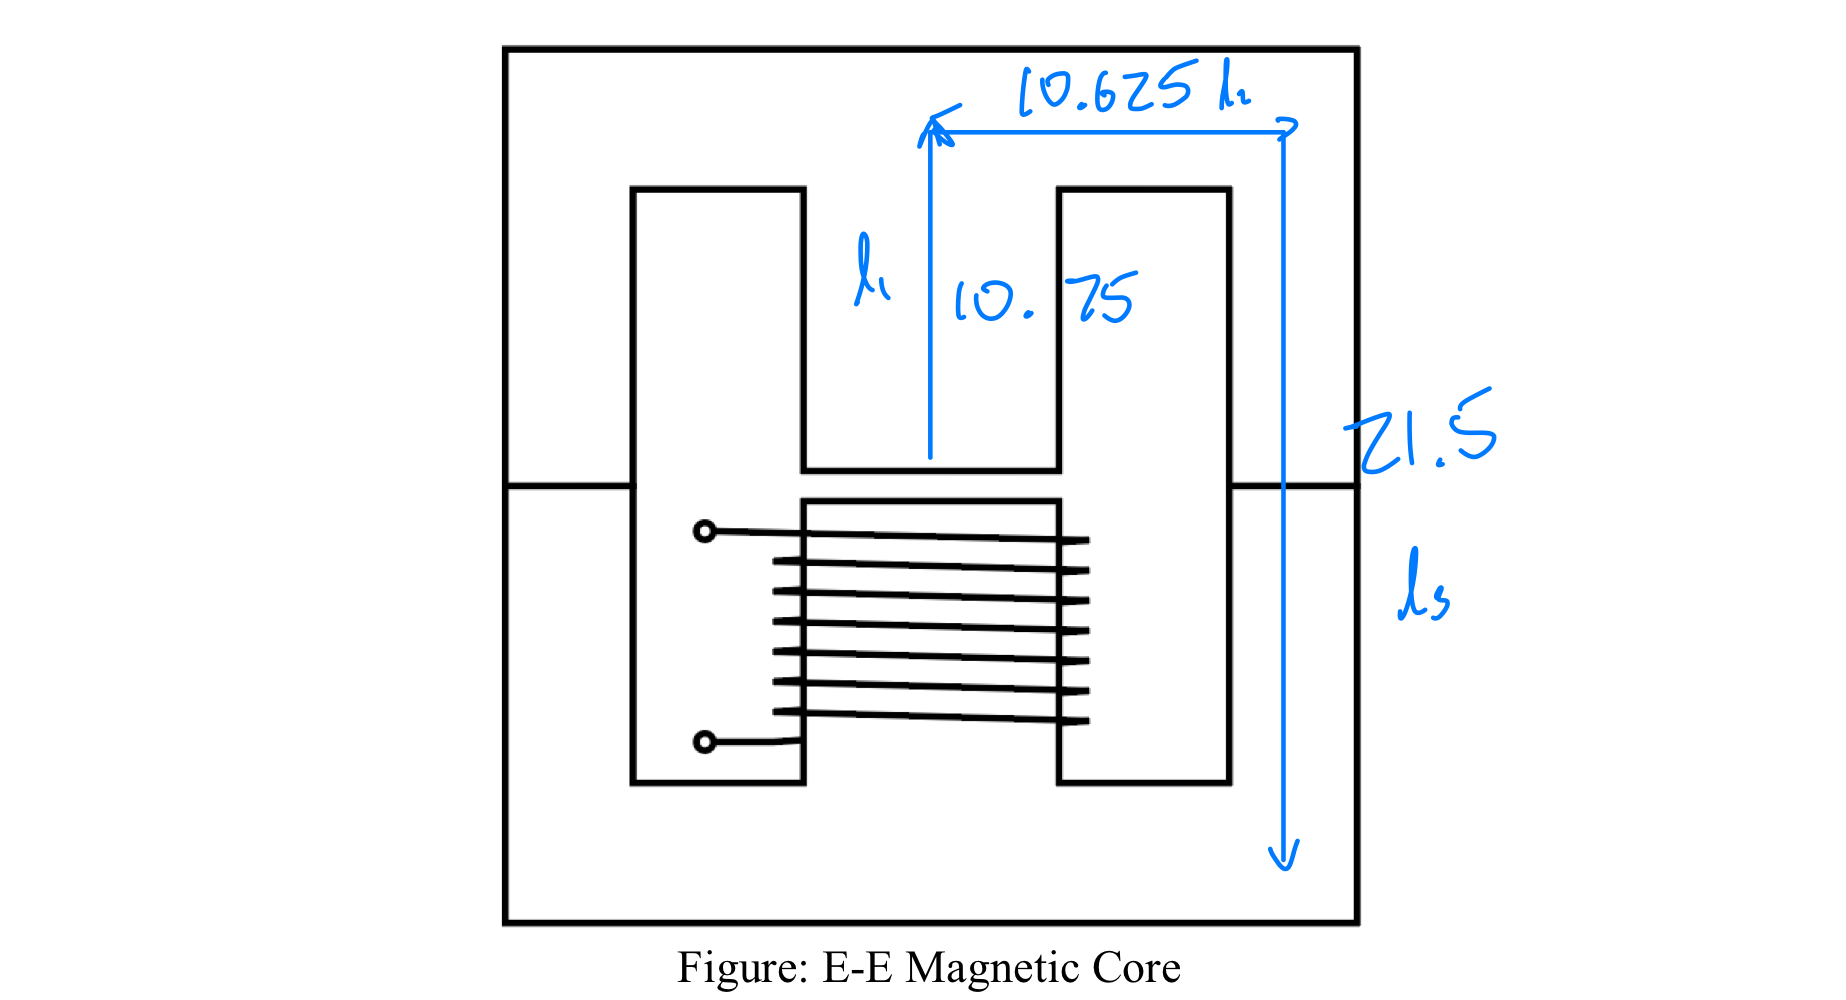
\includegraphics[width=0.65\textwidth]{q2.png}
    \label{Q2-img}
\end{figure}
The first business is to calculate the reluctance of the magnetic circuit.
\\$ h = 7.5mm$,  $\mu_e = 131$, $\mu_0 = 4\pi*10^{-7}$, $\mu_{ag} = 1$ \\
\\NOTE: For the permeability, I was unsure about whether to use $\mu_e = 1620$ or $\mu_e = 131$ because in the first case (1620) the result made more numerical sense however this permeability was marked for the ungapped model meanwhile the case of 131 was the gapped model but the results made less numerical sense.\\
\\Consider that $R_A = R_{A}^{'}$ where A and $A^'$ are the loop along the left and right segments respectively from the centre. Since circuit is symmetric they are equivalent.Further, our equivalent circuit looks like:
\begin{figure}[H]
    \centering
    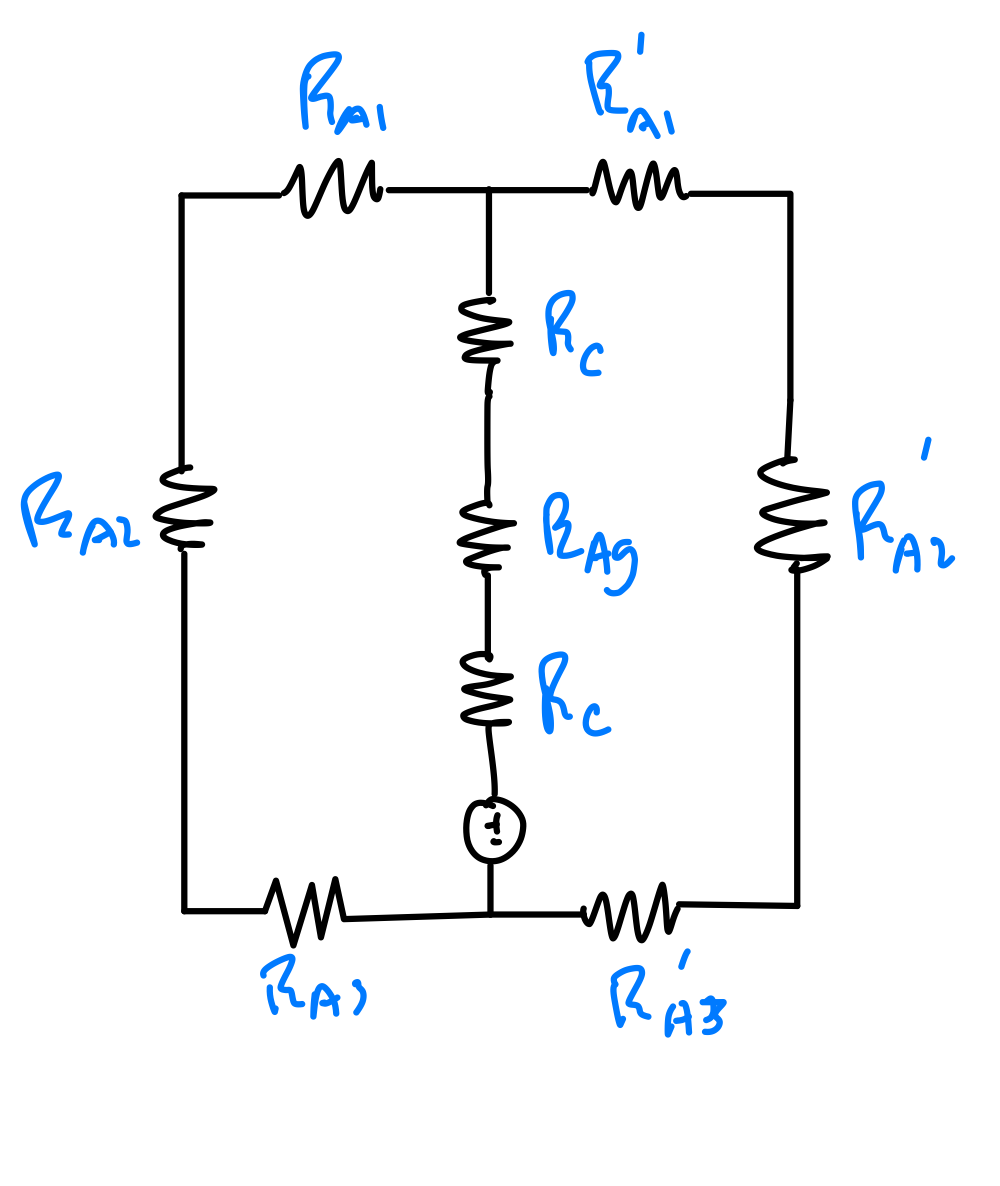
\includegraphics[width=0.5\textwidth]{Q2-eq-circ.png}
    \label{q2 - eq circuit}
\end{figure}
Moreover, the total reluctance can be calculated using the following:
\begin{align*}
    R_{total} &= (R_A || R_A') + R_C' = [R_A^{-1} + R_A'^{-1}]^{-1} + R_C' = \frac{1}{2}R_A + R_C'\\
    \rightarrow & R_A = R_A' = 2R_{A1} + R_{A2} \\
    \rightarrow & R_C' = 2R_C + R_{ag}
\end{align*}
Calculating all the sub-reluctances where: $R = \frac{l}{\mu_0 \mu_e A}$
\begin{align*}
    R_{A1} &= R_{A3} = \frac{10.625}{(4\pi*10^{-7})(131)(7.5*4.1*10^{-3})} = 2098952.7 [H^{-1}]\\
    R_{A2} &= \frac{21.5}{(4\pi*10^{-7})(131)(7.5*3.75*10^{-3})} = 4643706.6[H^{-1}]\\
    R_{C} &= \frac{10.75}{(4\pi*10^{-7})(131)(7.5^2*10^{-3})} = 1160926.6 [H^{-1}]\\
    R_{ag}&= \frac{1}{(4\pi*10^{-7})(1)(7.5^2*10^{-3})} = 7073553[H^{-1}]\\
    \mbox{Therefore we get the following:}\\
    R_A = R_A' = 8841612.0 [H^{-1}] & R_C' = 9395406.3 [H^{-1}]\\
    \mbox{And finally that: }\\
    R_{total} &= 13816212.3 [H^{-1}]
\end{align*}

\section*{Part a}
Calculate the reluctance of the magnetic circuit and $A_L$. Compare it with the value provided in the datasheet and comment on the reasons why they might differ. Add an illustration showing the equivalent electric circuit with the different reluctance found in the magnetic core.\\
\\To calculate $A_L$ we can use the following formula:
$A_L = \frac{1}{R_{total}} = 13816212.3^{-1} = 0.724 nH$\\
Note: the question insinuates that the units should be in [nH/$turn^2$] however from the datasheet and our leanings in class and tutorial I didn't find it to make sense.

\section*{Part b}
Calculate the value of the inductance obtained with 25 turns.\\
\\$L = \frac{N^2}{R} = \frac{25^2}{13816212.3} = 4.52*10^{-5}H$

\section*{Part c}
Based on the maximum flux density of the N87 magnetic material (consider T = 100$^{\circ}$C as the worst-case scenario), calculate the maximum current that should be allowed in this 25-turn inductor to avoid saturation.
\begin{align*}
    \phi &= \frac{N*i_{max}}{R_{total}}& \phi = BA = (390*10^{-3})(7.5*10^{-3})^2 \\
    \rightarrow i_{max}& = \frac{\phi * R_{total}}{N} = \frac{(390*10^{-3})(7.5*10^{-3})^2(13816212.3)}{25} \\
    i_{max} &= 12.12[A]
\end{align*}

\section*{Part d}
Explain what would happen to the reluctance of the magnetic circuit, and consequently inductance if this circuit is exceeded.\\
\\ If the circuits current is exceeded then the inductor becomes saturated meaning that it will act as a short circuit. As a result, the reluctance would significantly increase and the inductance is effectively zero.

\section{Question 3}
Using the circuit provided in the assignment sheet, a transformer with the following parameters connected to a square waveform voltage source of 50 percent duty cycle that alternates between +110V and -90V with a frequency of 1kHz.
\begin{figure}[H]
    \centering
    \includegraphics[width=0.75\textwidth]{Q3.png}
    \caption{Caption}
\end{figure}

\begin{center}
\begin{tabular}{ c c c c}
    $R_1 = 1 \Omega $ & $L_{l2} = L_{l3} = 5 \mu H$ & $L_{l1} = 0.1 mH$ & $R_2 = R_3 = 0.1 \Omega$ \\ & $R_m = 10k \Omega$ & $R_L = 5 \Omega$ & $L_m = 50mH$
\end{tabular}
\end{center}
\section*{Part a}
Calculate the DC component (average value) of the input current. What is the effect of this current on the secondary? How does this current affect the operation of the transformer.\\
\\We know that we are given the max and min voltage from the question therefore we can calculate $V_{avg}$:
\begin{align*}
    V_{avg} &= \frac{110 + (-90)}{2} = 10V
\end{align*}
Moreover, from the hint we also know that: $I_{avg} = \frac{V_0}{Z_{(\omega = 0)}} = \frac{10}{R_1 + R_m} \approx  \frac{10}{10k\Omega} = 1mA$ \\
\\
Moreover we know that $I_{avg,DC}$ does not induce any current in the secondary but without any back emf we see that current is large meaning that it drivers the transformers into saturation.

\section*{Part b}
Determine the approximate voltage waveforms at the two secondary windings taking the center point of the transformer as reference (0V point). Make the necessary assumptions and support them, to neglect elements as considered appropriate to facilitate the analysis.\\
\\From the hint, we know that $\frac{V_i}{V_j} = \frac{N_i}{N_j}$ so therefore we can derive that: $\frac{V_1}{V_2} = \frac{N_1}{N_2}$ and $\frac{V_1}{V_3} = \frac{N_1}{N_3}$ \\
Moreover, we had to make some key assumptions that: 
\begin{align*}
    &R_1, R_2, R_3, << R_M
    &L_{l1}, L_{l2}, L_{l3} << L_M
\end{align*}
\\ And as a result we will ignore $R_1, R_2, R_3$. Rearranging the above equations relating voltage and turns we can then derive each individual voltage.\\
\\Further recall that $V_{1,max} = 100V$ and $V_{1,min} = -100V$ and that $N_1=4, N_2=N_3 = 1$
\begin{align*}
    V_{2,max} &= \frac{N_2}{N_1}V_{1,max}=\frac{1}{4}*100 = 25V \\
    V_{2,min} &= \frac{N_2}{N_1}V_{1,min}=\frac{1}{4}*(-100) = -25V \\
    \mbox{And then for $V_3$:}\\
    V_{3,max} &= \frac{N_3}{N_1}V_{1,max}=\frac{1}{4}*100 = 25V \\
    V_{3,min} &= \frac{N_3}{N_1}V_{1,min}=\frac{1}{4}*(-100) = -25V \\
\end{align*}
Finally, the graphs for $V_2$ and $V_3$ look like this:
\begin{center}
    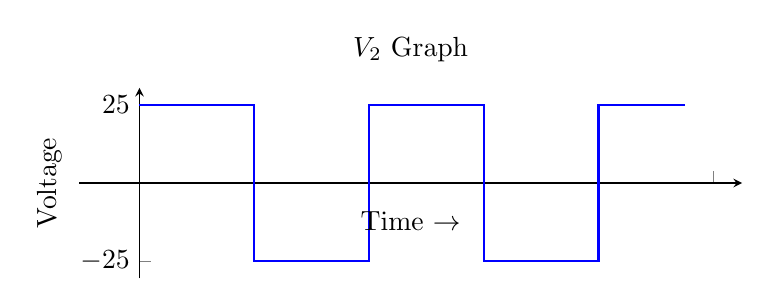
\begin{tikzpicture}
    \begin{axis}[
    width=10cm,
    height=4cm,
    x axis line style={-stealth},
    y axis line style={-stealth},
    title={$V_2$ Graph},
    xticklabels={},
    ymax = 30.5, xmax=5.25,
    axis lines*=center,
    ytick={-25,25},
    xlabel={Time $\rightarrow$},
    ylabel={Voltage}]
    \addplot+[thick,mark=none,const plot]
    coordinates
    {(0,25) (1,0) (1,-25) (2,0) (2,25) (3,25) (3,0) (3,-25) (4,-25) (4,0) (4,25) (4.75,25)};
    \end{axis}
    \end{tikzpicture}
\end{center}
\begin{center}
    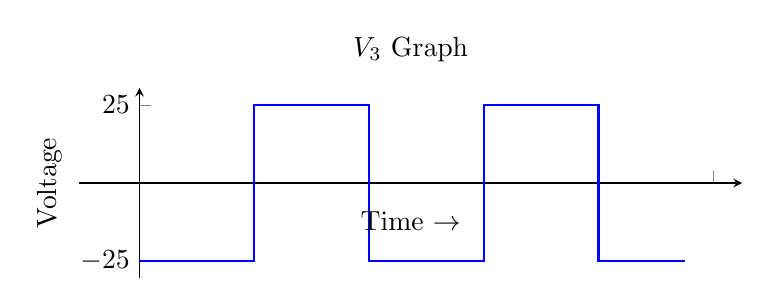
\begin{tikzpicture}
    \begin{axis}[
    width=10cm,
    height=4cm,
    x axis line style={-stealth},
    y axis line style={-stealth},
    title={$V_3$ Graph},
    xticklabels={},
    ymax = 30.5, xmax=5.25,
    axis lines*=center,
    ytick={-25,25},
    xlabel={Time $\rightarrow$},
    ylabel={Voltage}]
    \addplot+[thick,mark=none,const plot]
    coordinates
    {(0,-25) (1,0) (1,25) (2,0) (2,-25) (3,-25) (3,0) (3,25) (4,25) (4,0) (4,-25) (4.75,-25)};
    \end{axis}
    \end{tikzpicture}
\end{center}


\section*{Part c}
Determine the voltage and current waveforms and averages at the load resistor $R_L$ and indicate the conduction intervals of each diode.\\
\\ Recall that we use the same assumptions as in part b. With regards to the conduction intervals for each diode, it will be the corresponding half cycle. This is, that when $V_3$ and $V_2$ are negative, then $D_1$ and $D_2$ will conduct respectively. Further, to calculate $V_{load,avg}$ we can consider where the inductor is being shorted since there's a low conductance
\begin{align*}
    V_{load, avg} &= V_{2,max} * \frac{R_L}{R_2+R_L} = 25*\frac{5}{5+0.1} = 24.51V\\
    I_{load, avg} &= \frac{V_{avg}}{R_L} = \frac{24.51}{5} = 4.9A
\end{align*}
\\ Also, for the waveforms they are roughly straight lines similar to part b except near the times between the switching of voltage cycles where the inductors have yet to establish their magnetic fields.
\section*{Part d}
Simulate the complete circuit employing PSIM and compare the results with your calculations. Include relevant waveforms and plots obtained from the simulation.
\begin{figure}[H]
    \centering
    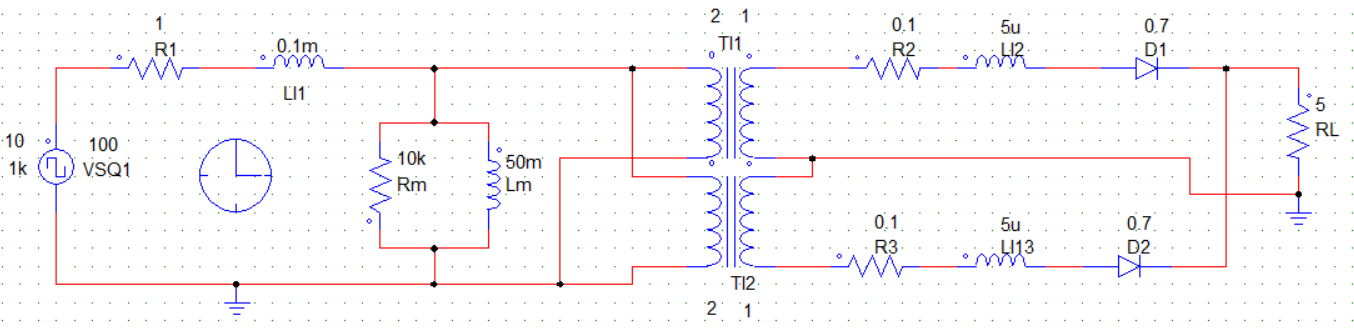
\includegraphics[width=0.85\textwidth]{q3d.png}
    \caption{Q3 PSIM}
\end{figure}
\begin{figure}[H]
    \centering
    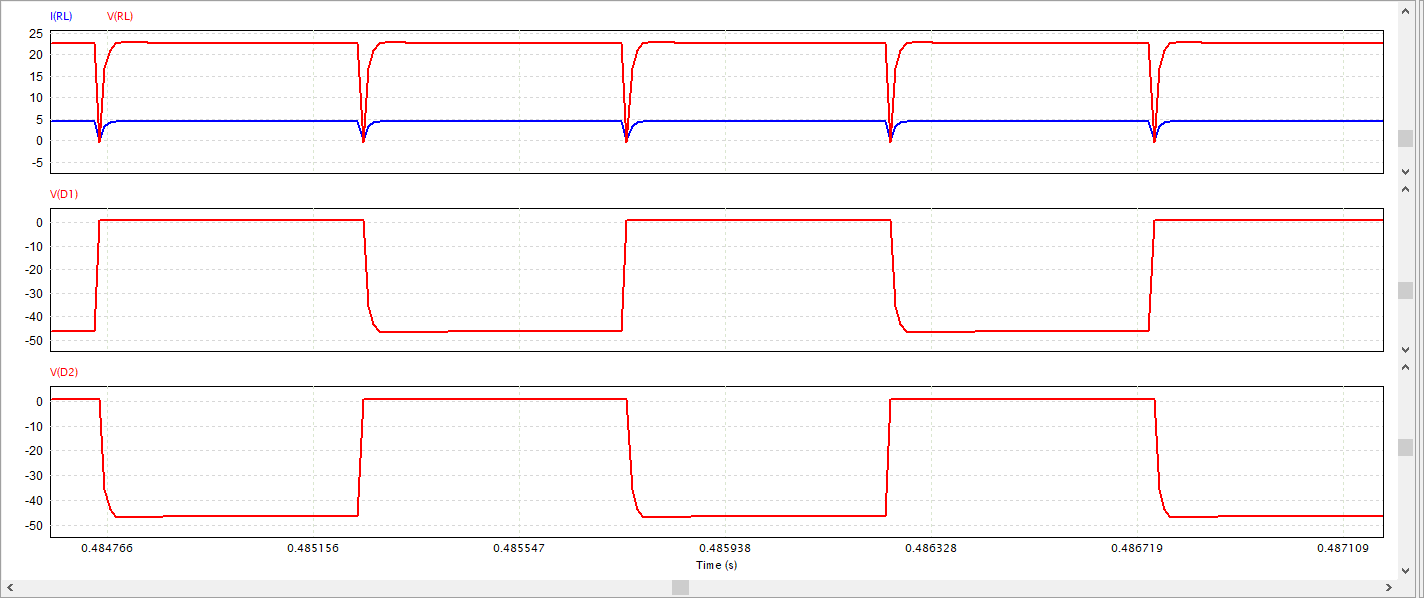
\includegraphics[width=1\textwidth]{q3d-f.png}
    \caption{Q3 Simulation results}
\end{figure}
From the recorded graphs we can see that there were a few slight differences. The simulated results are slightly less than the theoretical values since the simulation since my calculations neglected the transformer's internal resistance from the wires.
\begin{center}
    \begin{tabular}{|c | c c ||} 
    \hline
    Average values & $V_{load, avg}$[V]& $i_{load,avg}$ [A]\\
    \hline\hline
    Calculated & 24.51 & 4.51 \\
    \hline
    Simulated & 22.545 & 4.49 \\
    [1ex] 
    \hline
    \end{tabular}
\end{center}

\section*{Part e}
What is the effect of the leakage inductances and series resistances on the output voltage?\\
\\Leakage inductances result in a lower transmitted voltage through the transformer while series resistance also results in lower voltage outputs.

\section*{Part f}
Explain the physical phenomena that cause series resistances, leakage inductances, and magnetizing inductance and resistance.\\
\\series resistance reduces voltage output by dissipating power through small resistances in the wire coils of a real conductor. Meanwhile, leakage inductances lower transmitted voltage since transmitted voltage is directly related to the flux through the core. Thus, the leakage from the transformer is flux passing through the air.\\
\\Magnetizing resistance represents the total core losses and the magnetizing inductance represents magnetic flux in the core.

\end{document}